\section{Hilly Region Data Analysis}

The following code filters climate data for selected districts in Nepal’s hilly region and prepares it for a temperature distribution map.

\subsection*{Filtering Districts and Calculating Averages}

\begin{verbatim}
# Create a vector of districts to filter
districts_to_filter <- c("Arghakhanchi","Baglung",
"Baitadi", "Bhaktapur", "Chitwan","Dadeldhura",
"Dailekh", "Dhading", "Dhankuta",  "Dolpa", "Gorkha", 
"Gulmi", "Ilam", "Jumla","Kabhre", "Kaski", 
"Kathmandu", "Lalitpur", "Lamjung", 
"Makwanpur", "Myagdi", 
"Nuwakot", "Okhaldhunga", "Palpa", "Parbat", 
"Rukum", "Salyan", "Sindhuli", "Surkhet",
"Syangja")

# Filter the dataset to only include these districts
filtered_hilly_data <- subset(df_climate, District %in% districts_to_filter)

dim(filtered_hilly_data)
# 413076 25  # example output rows and columns
\end{verbatim}

\subsection*{Geoplot for Temperature Distribution in Hilly Region}

\begin{verbatim}
# Calculate average temperature per district
plot_hilly <- filtered_hilly_data %>%
  group_by(District) %>%
  summarise(
    avg_temp = mean(Temp_2m, na.rm = TRUE),
    avg_precip = mean(Precip, na.rm = TRUE),
    Latitude = first(Latitude),
    Longitude = first(Longitude)
  )

# Merge temperature data with spatial data
nepal_temp_hilly <- left_join(nepal_districts, plot_hilly, by = "District")
\end{verbatim}

% Figure here----------------------------
\begin{figure}[h]
\centering
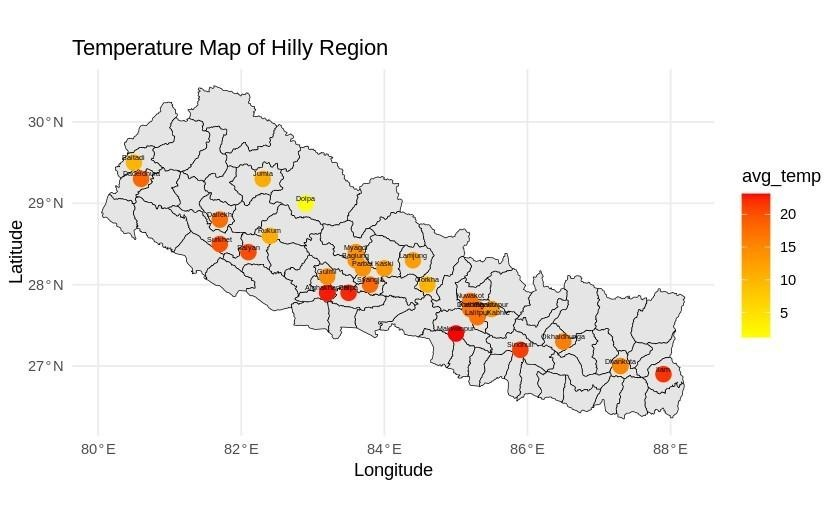
\includegraphics[width=0.6\textwidth]{figures/hilly_map.jpg}
\caption{Temperature Distribution in Nepal using Geoplot
}
\end{figure}

\subsection*{Temperature vs Humidity in the Hilly Region}

The following scatter plot visualizes the relationship between temperature and humidity across districts in the hilly region, colored by season:

\begin{verbatim}
ggplot(filtered_hilly_data, aes(x = Temp_2m, y = Humidity_2m)) +
  geom_point(aes(color = Season), alpha = 0.6) +
  theme_minimal() +
  labs(title = "Temperature vs Humidity in the Hilly Region",
       x = "Temperature (°C)",
       y = "Humidity (%)")
\end{verbatim}

% figure here----------------------------
\begin{figure}[h]
    \centering
    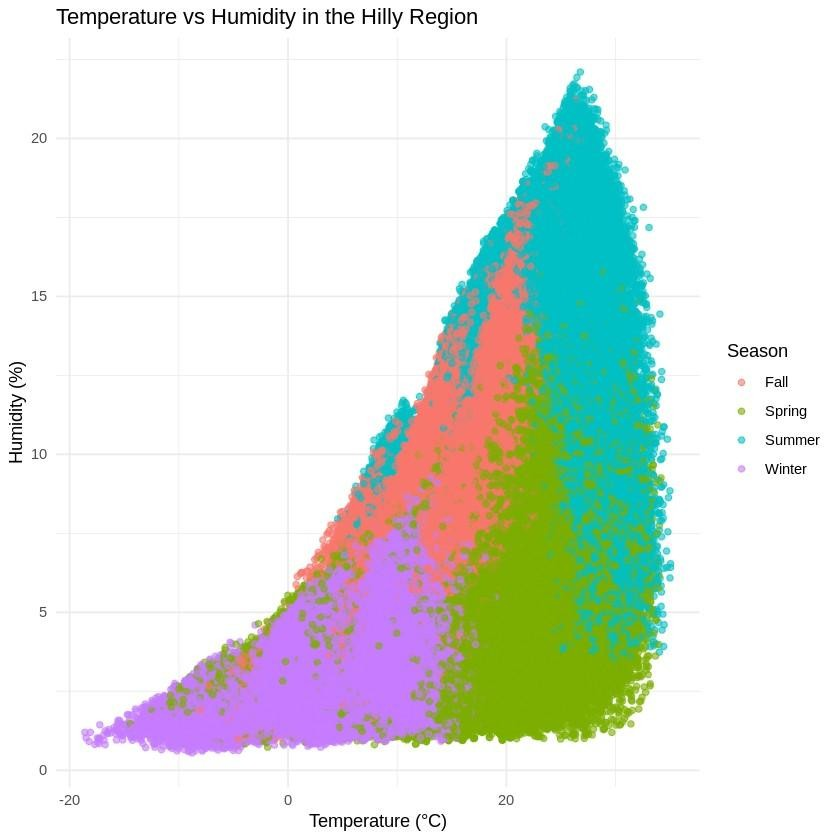
\includegraphics[width=0.5\textwidth]{figures/scatter_hilly.jpg}
    \caption{Scatterplot showing temperature vs humidity according to season}
\end{figure}

\subsubsection*{Insights from Temperature vs Humidity Plot}

\begin{itemize}
    \item A clear positive correlation is observed: higher temperatures generally correspond to higher humidity levels.
    \item Summer shows the highest humidity values, especially above 20\% humidity at moderate to high temperatures.
    \item Winter has the lowest humidity values, often below 10\% even at lower temperatures.
    \item Fall and Spring seasons occupy the middle humidity range, suggesting transitional moisture conditions.
    \item Humidity increases non-linearly with temperature, indicating stronger moisture-holding capacity at warmer temperatures.
    \item A dense clustering of points in summer highlights more consistent humid conditions during that season.
    \item Wider spread of points in winter and spring indicates greater variability in humidity for similar temperature levels.
\end{itemize}

\subsection*{Average Precipitation by District}

\begin{verbatim}
avg_precip_by_district <- filtered_hilly_data %>%
  group_by(District) %>%
  summarise(avg_precip = mean(Precip, na.rm = TRUE))

ggplot(avg_precip_by_district, aes(x = reorder(District, -avg_precip),
 y = avg_precip)) +
  geom_bar(stat = "identity", fill = "skyblue") +
  theme_minimal() +
  labs(title = "Average Precipitation by District",
       x = "District", y = "Average Precipitation") +
  theme(axis.text.x = element_text(angle = 90, hjust = 1))
\end{verbatim}

% Figure here----------------------------
\begin{figure}[h]
    \centering
    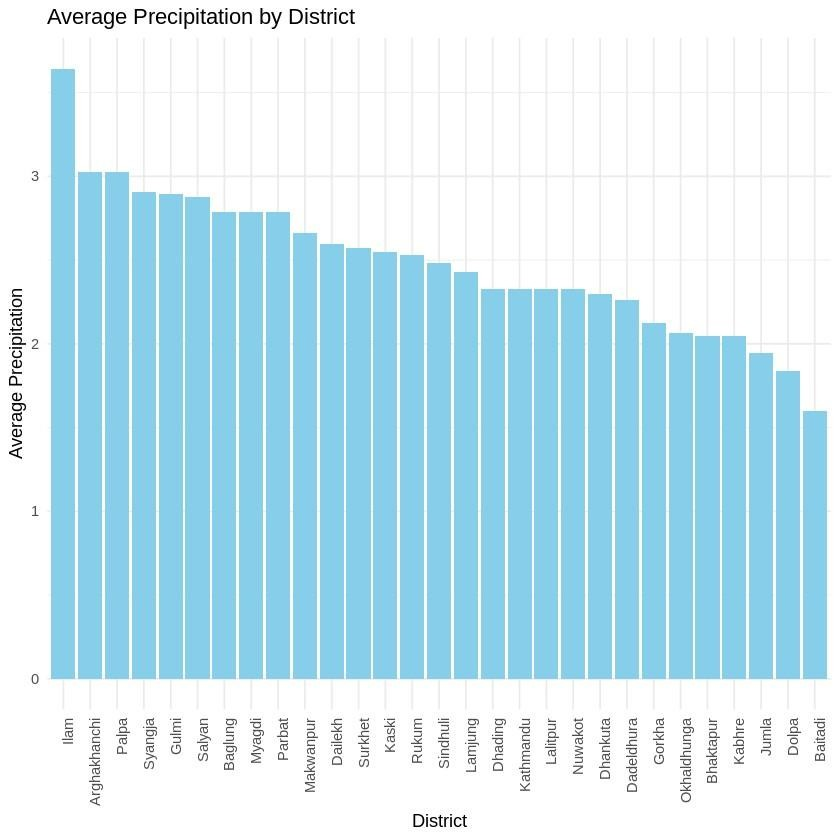
\includegraphics[width=0.5\textwidth]{figures/bar_hilly.jpg}
    \caption{Bar Chart of Average Precipitation in Hilly Region Districts}
\end{figure}

\subsection*{Boxplot of Seasonal Precipitation in Hilly Districts}

\begin{verbatim}
ggplot(filtered_hilly_data, aes(x = Season, y = Precip, fill = Season)) +
  geom_boxplot() +
  labs(title = "Seasonal Precipitation in Hilly Districts",
       x = "Season", y = "Precipitation (mm)") +
  theme_minimal()
\end{verbatim}

% Figure here-----------------------------
\begin{figure}[h]
    \centering
    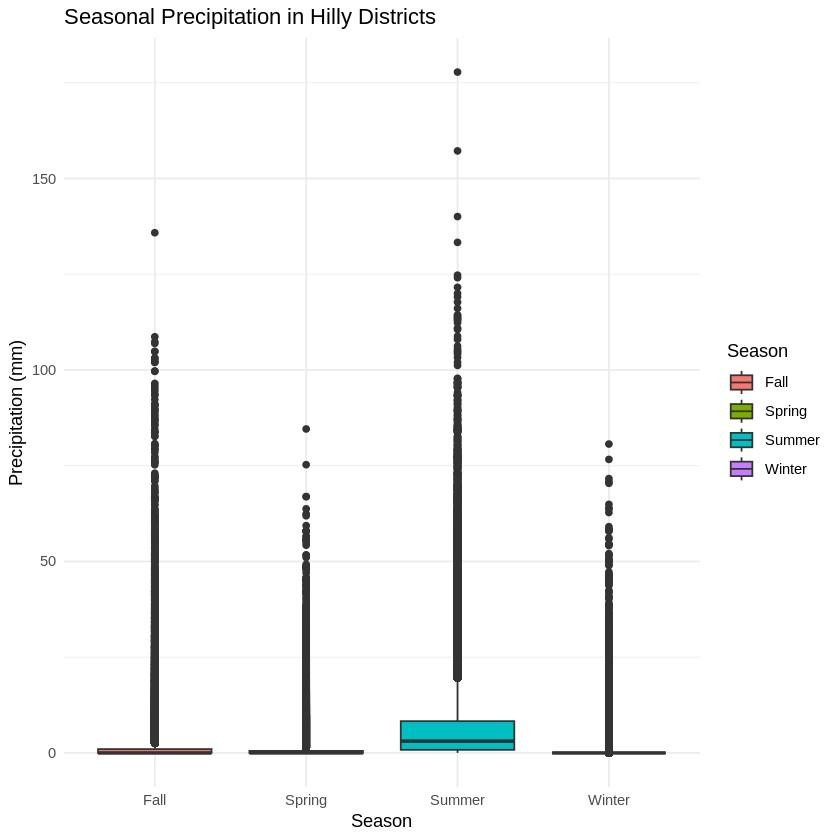
\includegraphics[width=0.5\textwidth]{figures/box_hilly.jpg}
    \caption{Seasonal Precipitation Distribution in Hilly Districts}
\end{figure}

\subsubsection*{Insights from Seasonal Precipitation Plot}

\begin{itemize}
    \item Summer records the highest median and variability in precipitation, indicating it as the peak rainy season.
    \item Spring, Fall, and Winter show comparatively lower median precipitation, clustered near zero.
    \item Despite low medians, all seasons exhibit outliers with precipitation events exceeding 100 mm.
    \item The box for Summer is significantly taller, suggesting a broader interquartile range and more frequent moderate to heavy rainfalls.
    \item Fall and Winter have tight boxes with few extreme outliers, indicating rare but intense rain events.
    \item Spring shows almost no visible box, suggesting highly concentrated low precipitation with sporadic extremes.
    \item Overall, precipitation in hilly districts is highly seasonal, with summer dominating rainfall contributions.
\end{itemize}

\subsection*{Density Plot of Relative Humidity Across Hilly Districts}

\begin{verbatim}
ggplot(filtered_hilly_data, aes(x = RH_2m, fill = District)) +
  geom_density(alpha = 0.4) +
  labs(title = "Humidity Distribution Across Hilly Districts",
       x = "Relative Humidity (%)", y = "Density") +
  theme_minimal()
\end{verbatim}

\begin{figure}[h]
    \centering
    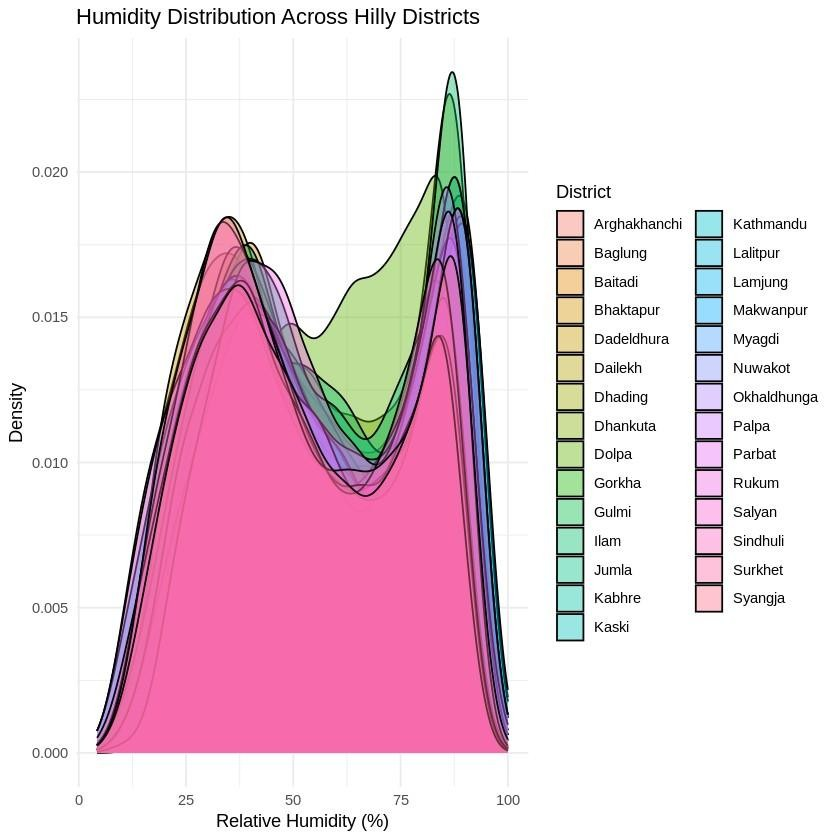
\includegraphics[width=0.5\textwidth]{figures/humid_hilly.jpg}
    \caption{Humidity Distribution Across Hilly Districts}
\end{figure}

\subsubsection*{Insights from Humidity Distribution}

\begin{itemize}
    \item The distribution is bimodal, indicating distinct dry and wet seasonal patterns.
    \item High relative humidity levels (75–90\%) are common across many districts.
    \item Districts like Rukum show broader density curves, suggesting higher variability in humidity.
    \item Districts such as Kathmandu and Dhankuta have sharper peaks, indicating more stable humidity conditions.
    \item Overlapping curves among districts point to similar climatic conditions in the hilly region.
    \item Tails extending towards 0\% and 100\% imply the occurrence of rare extreme humidity events.
    \item These patterns help identify humidity-prone areas useful for agricultural and climatic planning.
\end{itemize}

\subsection*{Extreme Precipitation Analysis in Hilly Regions}

Understanding extreme rainfall events is crucial for disaster preparedness, especially in hilly terrains where intense precipitation can trigger flash floods and landslides. This section presents an analysis of high-impact rainfall events in such regions based on the 95th percentile threshold.

\subsubsection*{Monthly Precipitation Trends}

We begin by computing average monthly precipitation for each year to examine seasonal variation.

\begin{verbatim}
monthly_precip_hilly <- filtered_hilly_data %>%
  group_by(Month_Number, Year = as.numeric(format(Date, "%Y"))) %>%
  summarize(Avg_Precip = mean(Precip, na.rm = TRUE))
\end{verbatim}

\subsubsection*{Defining Extreme Rainfall Events}

To isolate extreme rainfall events, we compute the 95th percentile of all precipitation values. Events exceeding this threshold are classified as extreme.

\begin{verbatim}
# Calculate the 95th percentile of Precipitation
extreme_threshold <- quantile(filtered_hilly_data$Precip, 0.95, na.rm = TRUE)

# Filter the extreme events
extreme_events_hilly <- filtered_hilly_data %>%
filter(Precip > extreme_threshold)

print(extreme_threshold)

95%
13.51
\end{verbatim}

\subsubsection*{Yearly Trend of Extreme Events}

We extract the year from each event and calculate the yearly frequency of extremes to visualize how often such events occur over time.

\begin{verbatim}
# Extract year and count extreme events per year
extreme_events_hilly$Year <- format(extreme_events_hilly$Date, "%Y")
yearly_extreme <- extreme_events_hilly %>%
group_by(Year) %>%
  summarize(Count = n())

# Plot yearly frequency
ggplot(yearly_extreme, aes(x = as.numeric(Year), y = Count)) +
geom_line() +
geom_point() +
labs(
  title = "Yearly Frequency of Extreme Precipitation Events",
  x = "Year",
  y = "Number of Extreme Events")
\end{verbatim}

% Figure here-----------------------------
\begin{figure}[h]
    \centering
    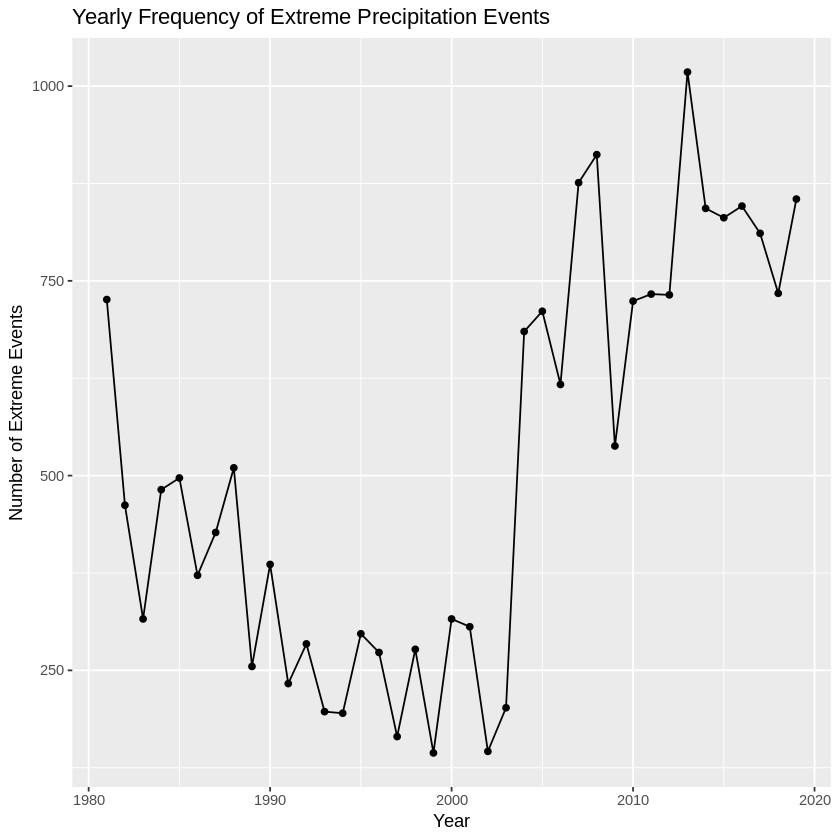
\includegraphics[width=0.5\textwidth]{figures/trend_hilly.jpg}
    \caption{Yearly Frequency of Extreme Precipitation Events}
\end{figure}

\subsubsection*{Yearly Trends}

\begin{itemize}
    \item Low and fluctuating frequency of extreme events from 1980 to early 2000s.
    \item Sharp increase in events post-2003, with a peak around 2013.
    \item Suggests rising climate variability and increased flood risk in recent decades.
\end{itemize}

\subsubsection*{Monthly Distribution of Extreme Events}

To identify seasonal flood risk, we count the number of extreme events in each month and visualize the distribution.

\begin{verbatim}
# Count extreme events per month
monthly_extremes <- extreme_events_hilly %>%
group_by(Month_Label) %>%
  summarize(Count = n())

# Plot the counts
ggplot(monthly_extremes, aes(x = Month_Label, y = Count)) +
geom_bar(stat = "identity", fill = "red") +
labs(
  title = "Number of Extreme Events Per Month",
  x = "Month", 
  y = "Count of Extreme Events")
\end{verbatim}

% Figure here-----------------------------
\begin{figure}[h]
    \centering
    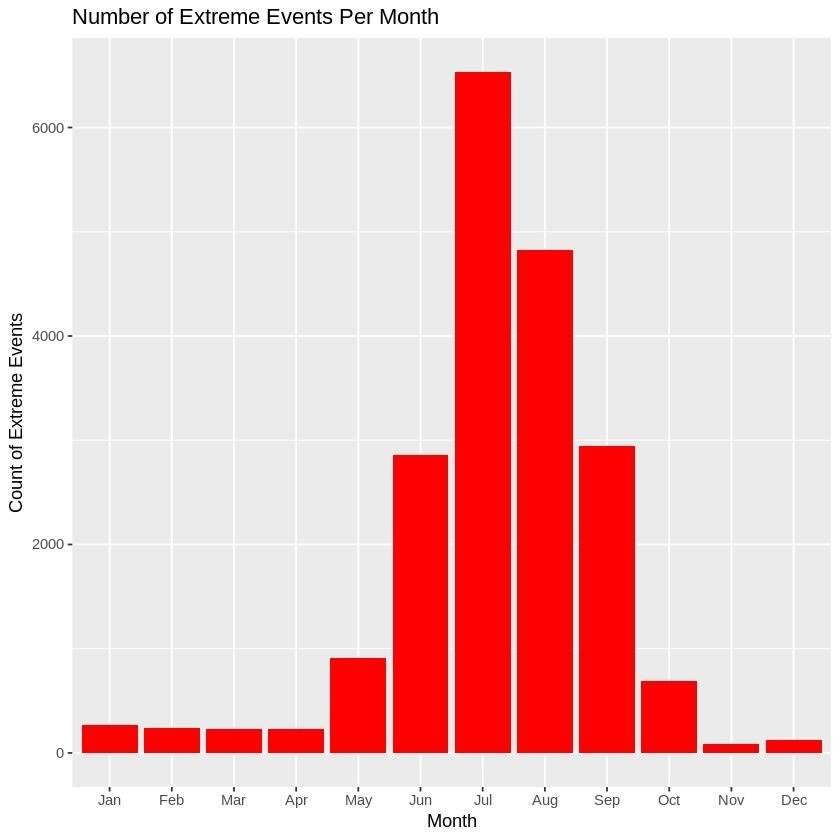
\includegraphics[width=0.5\textwidth]{figures/extreme_hilly.jpg}
    \caption{Number of Extreme Precipitation Events Per Month}
\end{figure}

\subsubsection*{Monthly Patterns}

\begin{itemize}
    \item Highest number of extreme events observed in July, followed by August and June.
    \item May and September show moderate activity—transitional monsoon months.
    \item Winter and spring months (November–April) show minimal extreme events.
\end{itemize}

\section*{Conclusion}

The analysis clearly highlights both a temporal increase in extreme rainfall events over the years and a strong seasonal concentration during the monsoon months. These findings emphasize the need for targeted flood preparation strategies, especially from June to September, and call for continuous monitoring and adaptation planning to improve climate resilience in vulnerable regions.

